% Made up for the tikra gallery: the line through two points and its slope. In the playground,
% drag P or Q.
\begin{tikzpicture}[scale=0.8]
  \def\px{-2}  % x of P, -4..4:0.1
  \def\py{-1}  % y of P, -4..4:0.1
  \def\qx{3}   % x of Q, -4..4:0.1
  \def\qy{2}   % y of Q, -4..4:0.1
  \useasboundingbox (-5.4,-5.4) rectangle (5.6,5.6);
  \draw[help lines] (-5,-5) grid (5,5);
  \draw[->] (-5.2,0) -- (5.3,0) node[right] {$x$};
  \draw[->] (0,-5.2) -- (0,5.3) node[above] {$y$};
  \coordinate (P) at (\px,\py);
  \coordinate (Q) at (\qx,\qy);
  \begin{scope}
    \clip (-5,-5) rectangle (5,5);
    \draw[very thick, teal!70!black, shorten <=-20cm, shorten >=-20cm] (P) -- (Q);
  \end{scope}
  \draw[dashed, orange!85!black] (P) -- (Q|-P) node[midway, below] {$\Delta x$} -- (Q) node[midway, right] {$\Delta y$};
  \fill (P) circle (2.5pt) node[below left] {$P$};
  \fill (Q) circle (2.5pt) node[above left] {$Q$};
  \pgfmathsetmacro\m{(\qy-\py)/(\qx-\px+0.0001)}
  \node[fill=white, inner sep=2pt, anchor=north west] at (-4.9,4.9) {slope $m = \dfrac{\Delta y}{\Delta x} = \pgfmathprintnumber[fixed, precision=2]{\m}$};
\end{tikzpicture}
